
\documentclass[a4paper,12pt]{article} 


\usepackage[T2A]{fontenc}			% кодировка
\usepackage[utf8]{inputenc}			% кодировка исходного текста
\usepackage[english,russian]{babel}	% локализация и переносы


% Математика
\usepackage{amsmath,amsfonts,amssymb} 

% Картинки
\usepackage{graphicx}
\graphicspath{{images/}}

%Заговолок
\usepackage[left=2cm,right=2cm,
    top=0cm,bottom=0cm,bindingoffset=0cm]{geometry}


\newcounter{first}
\renewcommand{\thefigure}{\arabic{first}.\arabic{figure}} 

\begin{document} % начало документа
\setcounter{figure}{0}
\setcounter{first}{1}
\renewcommand{\figurename}{График}

\begin{figure}[htpb!]
\centering
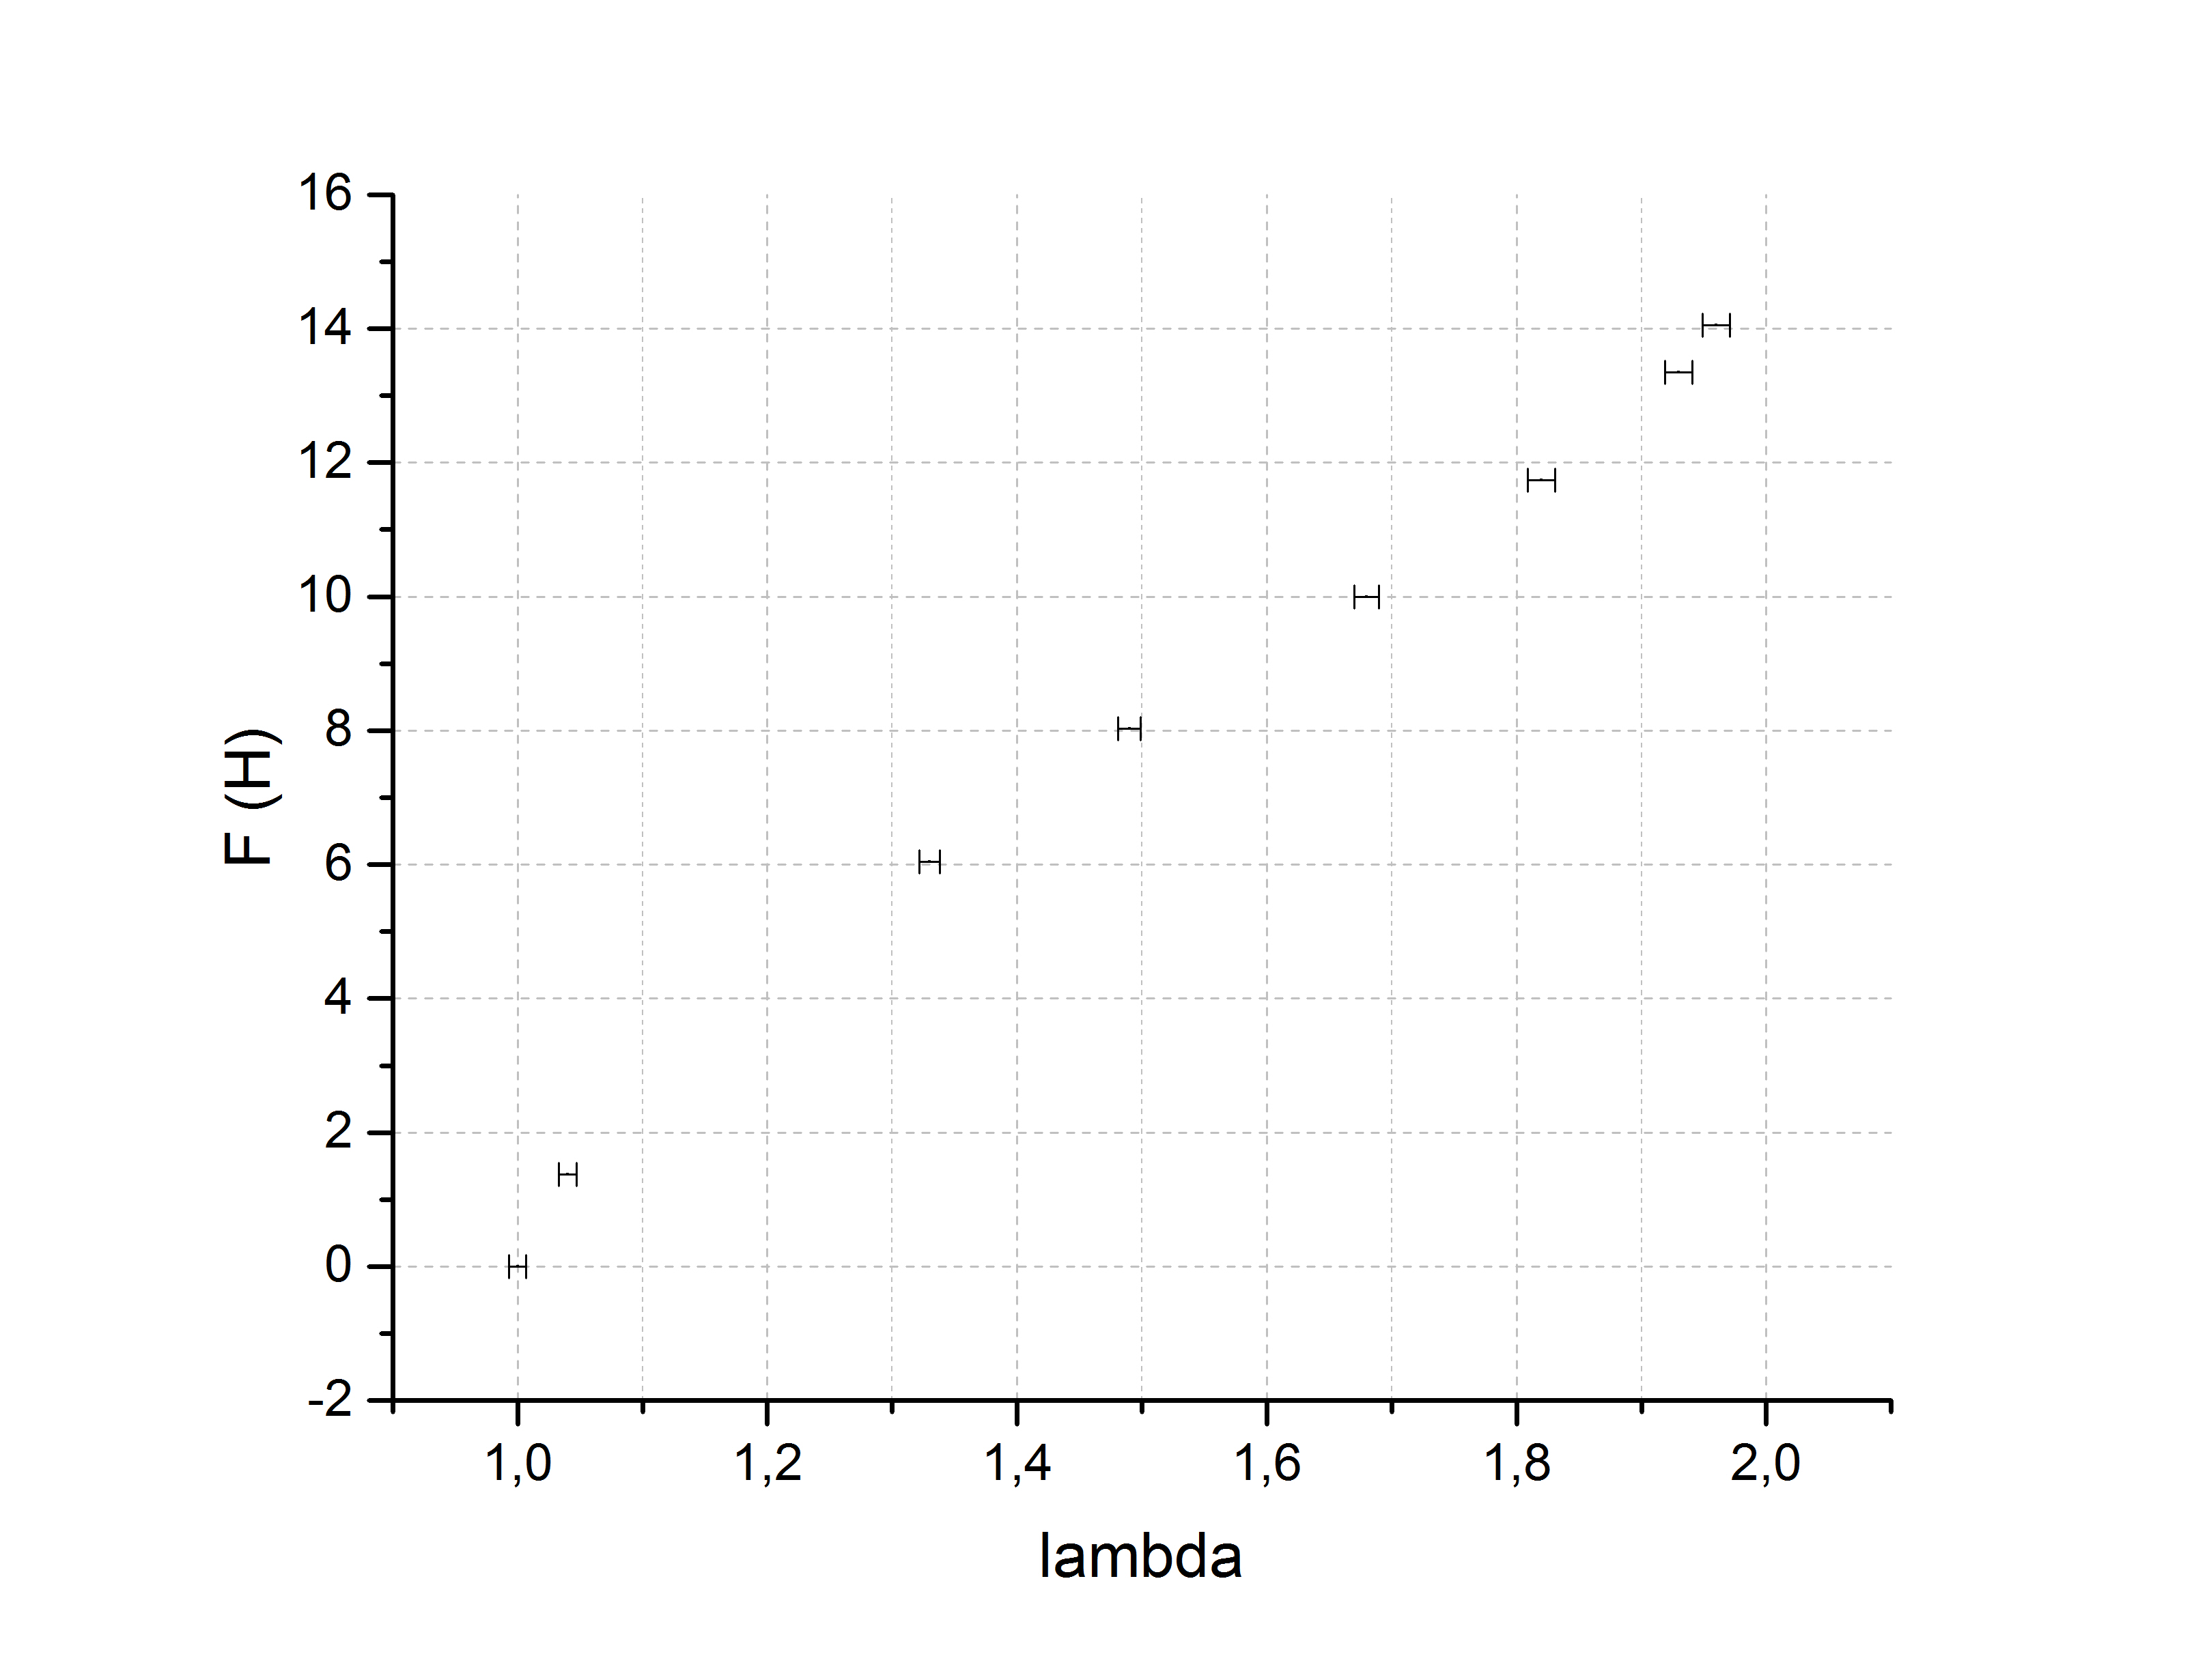
\includegraphics[width=150mm]{graph1_1.jpg}
\caption{Зависимость приложенной силы от относительного растяжения $\lambda$}
\end{figure}

\begin{figure}[htpb!]
\centering
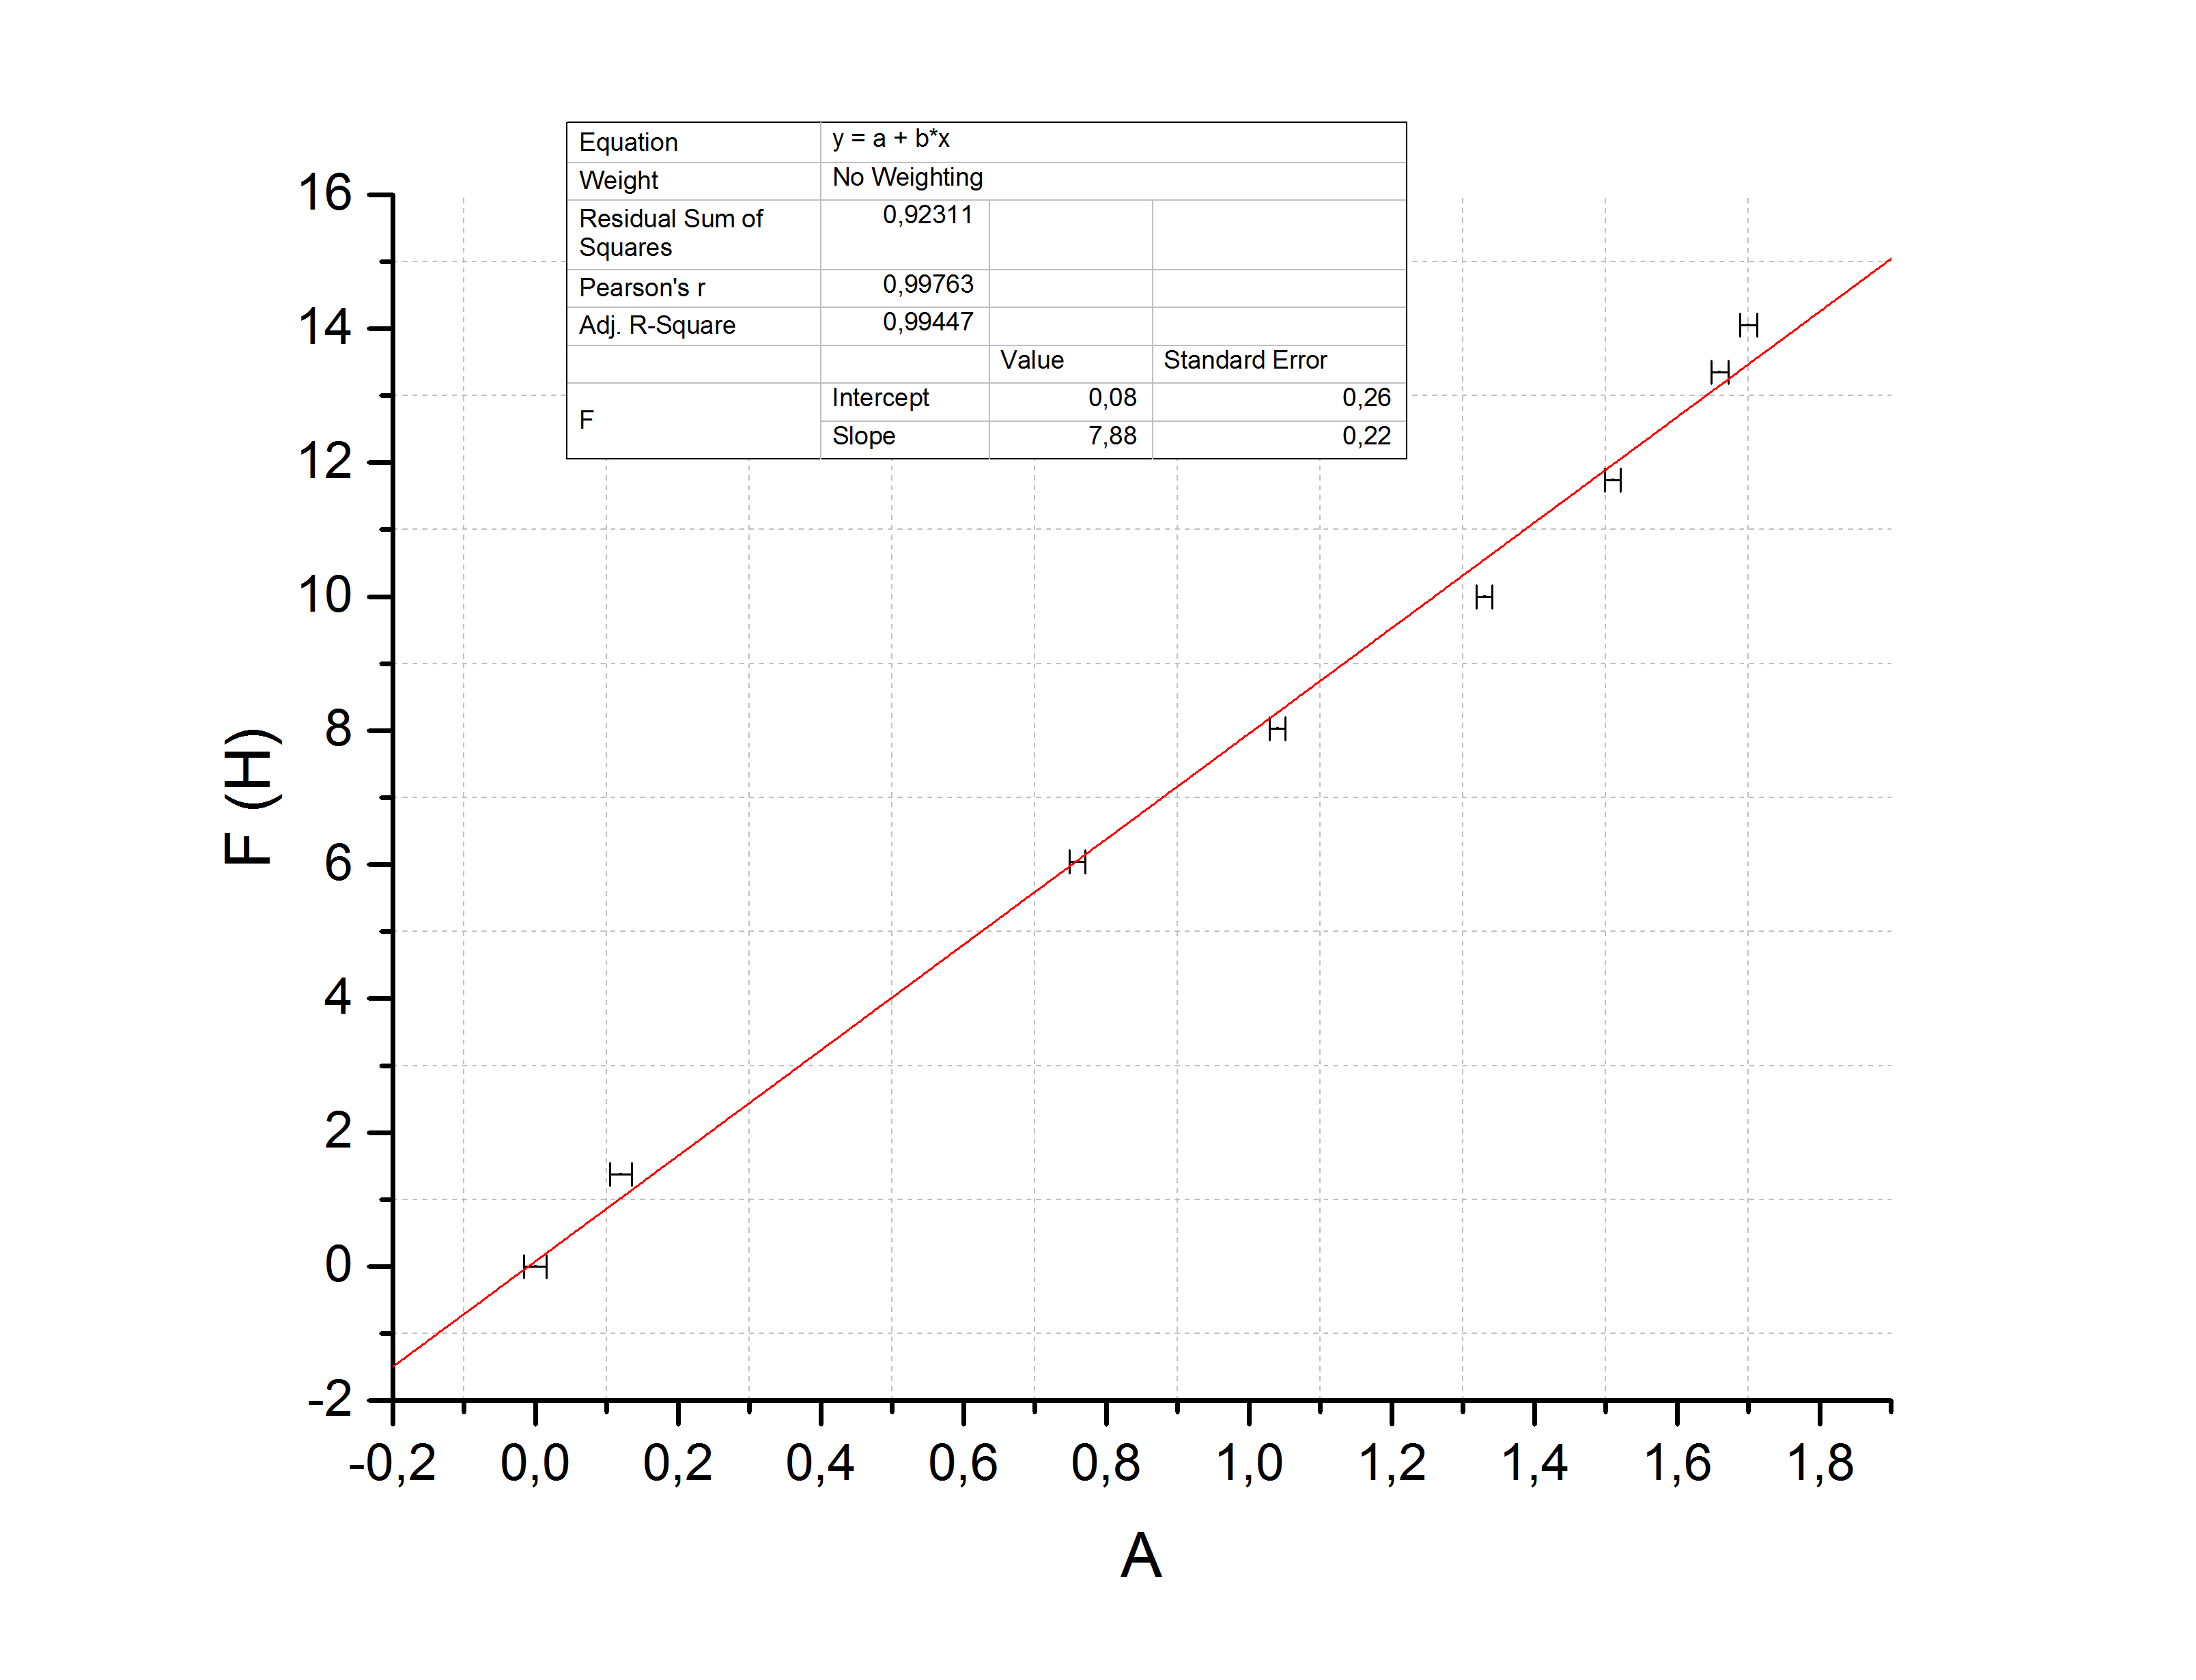
\includegraphics[width=150mm]{graph1_2.jpg}
\caption{Зависимость приложенной силы от величины $\lambda - \frac{1}{\lambda^2}$ и её аппроксимация }
\end{figure}

\stepcounter{first}
\setcounter{figure}{0} 

\begin{figure}[htpb!]
\centering
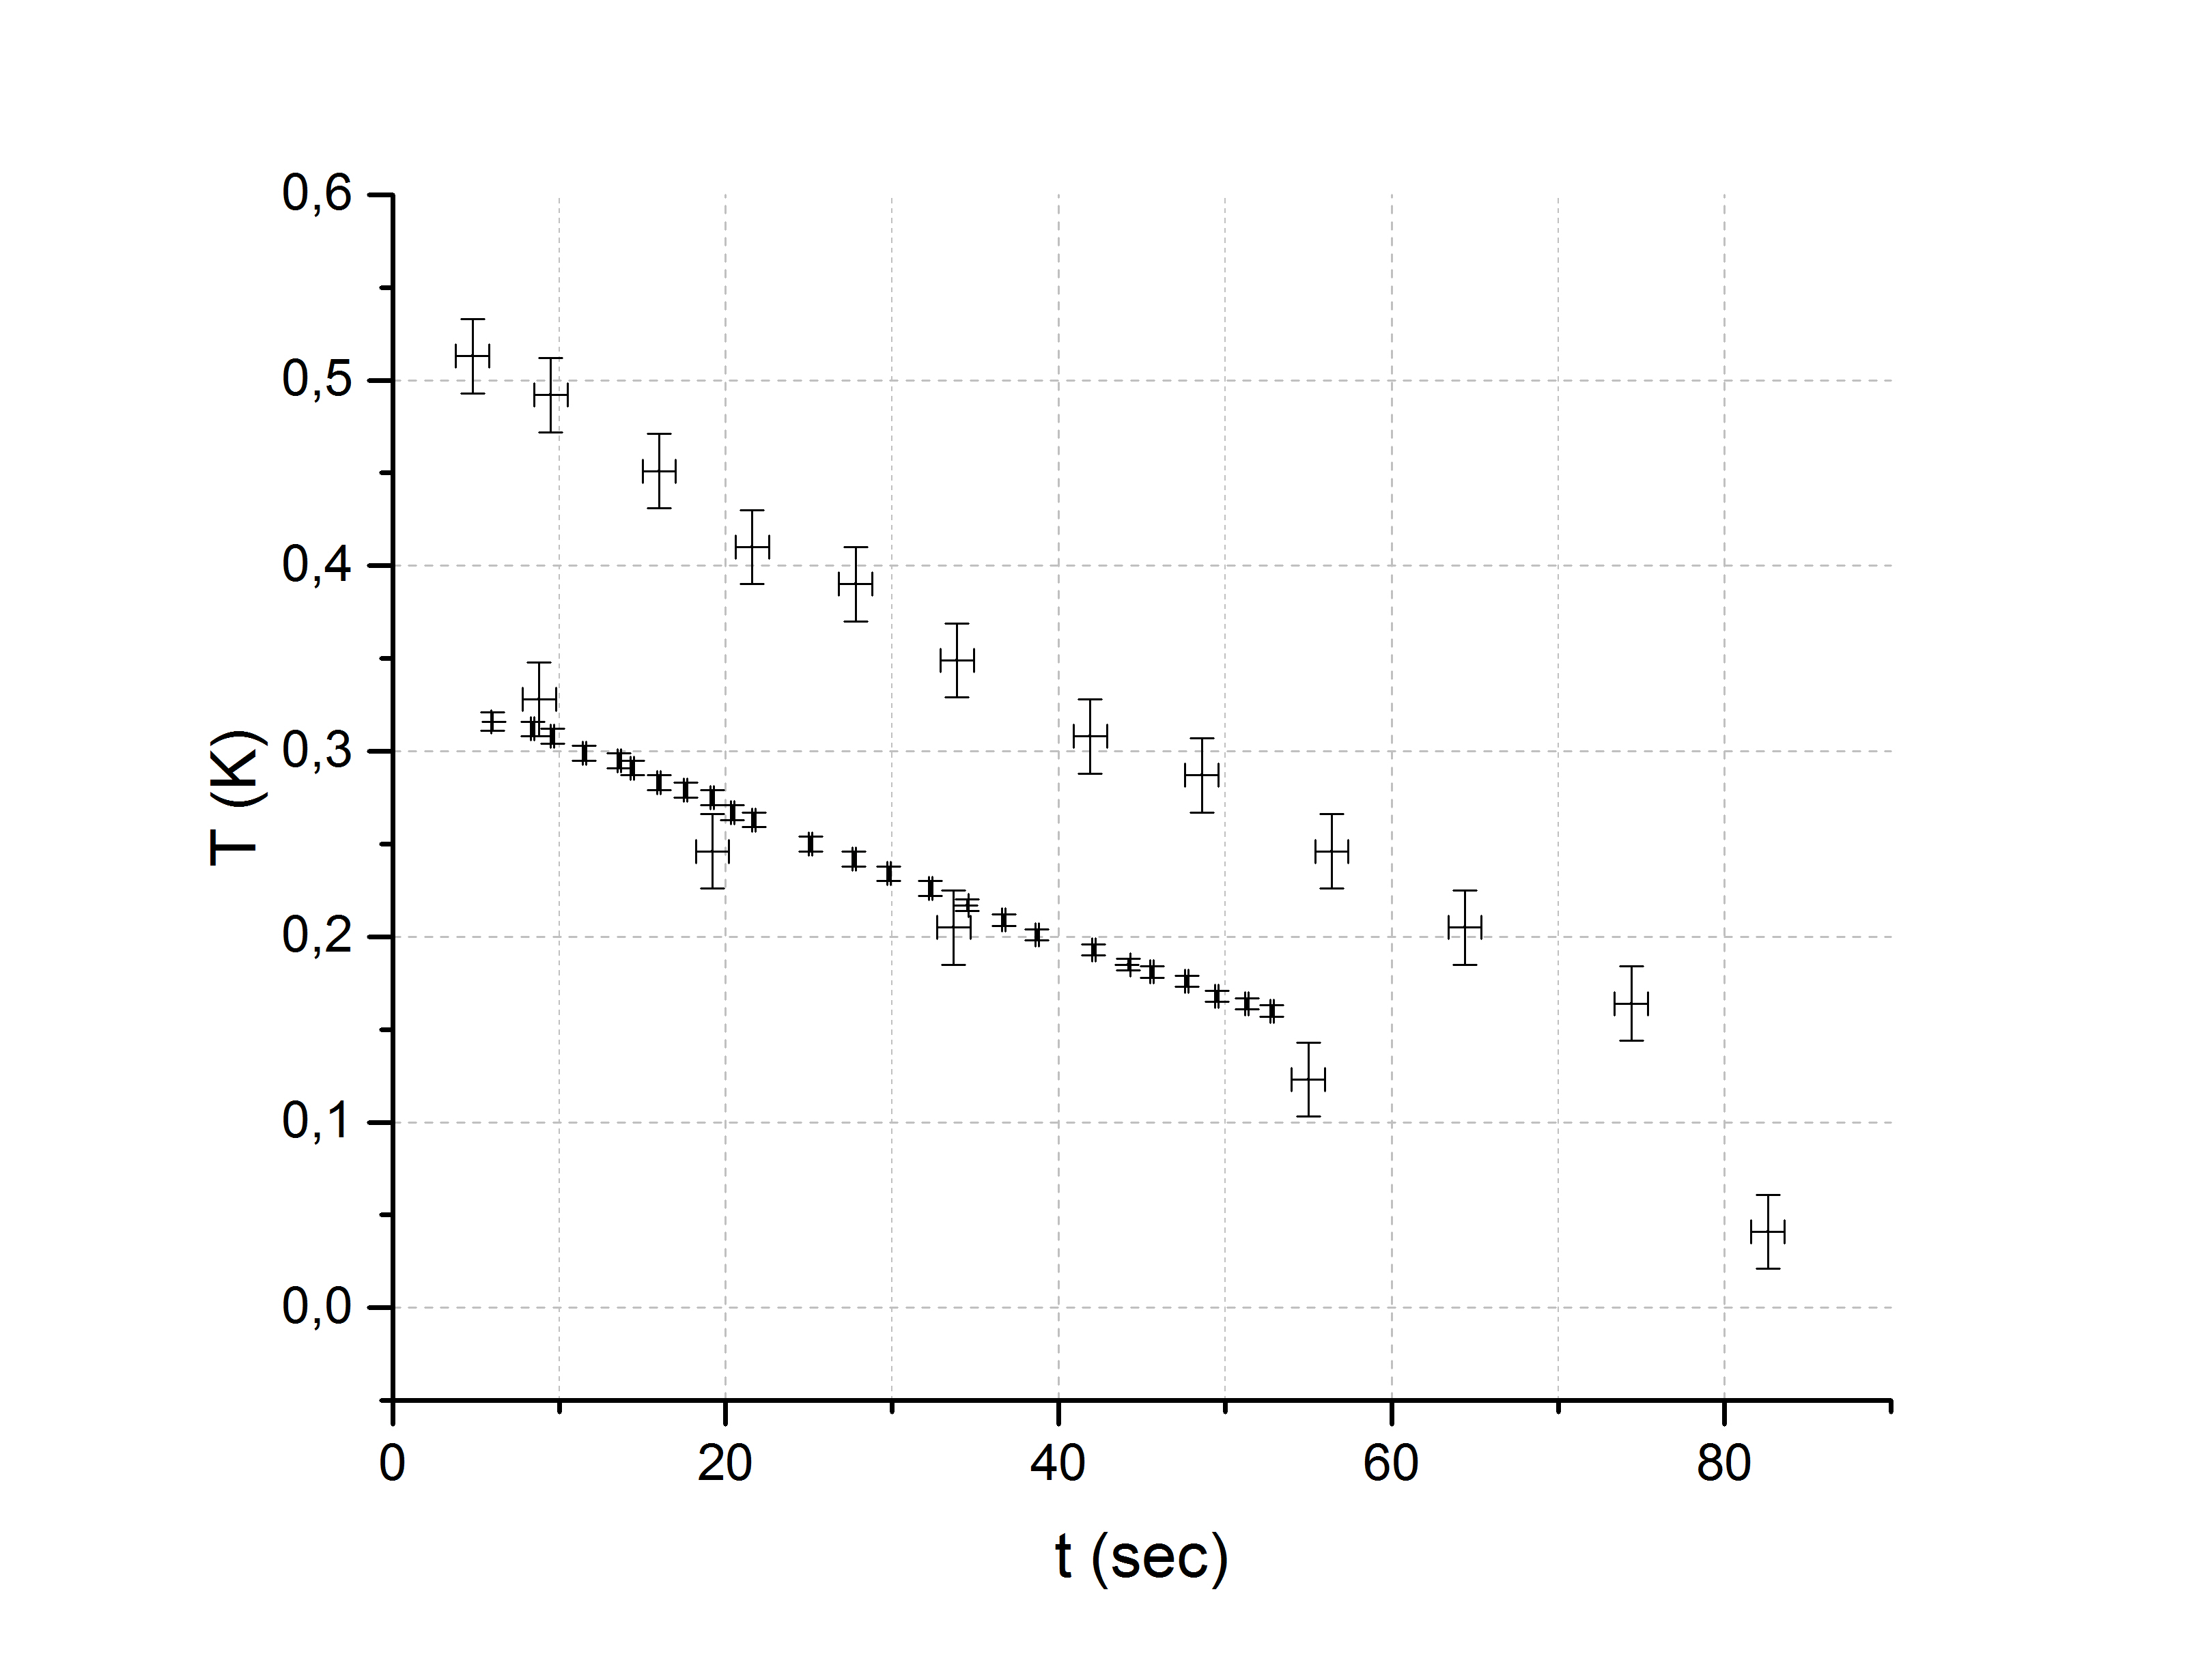
\includegraphics[width=150mm]{graph2_1.jpg}
\caption{Зависимость разницы температур резинки и воздуха от времени в трёх экспериментах при остывании резины после её резкого растяжения}
\end{figure}

\begin{figure}[htpb!]
\centering
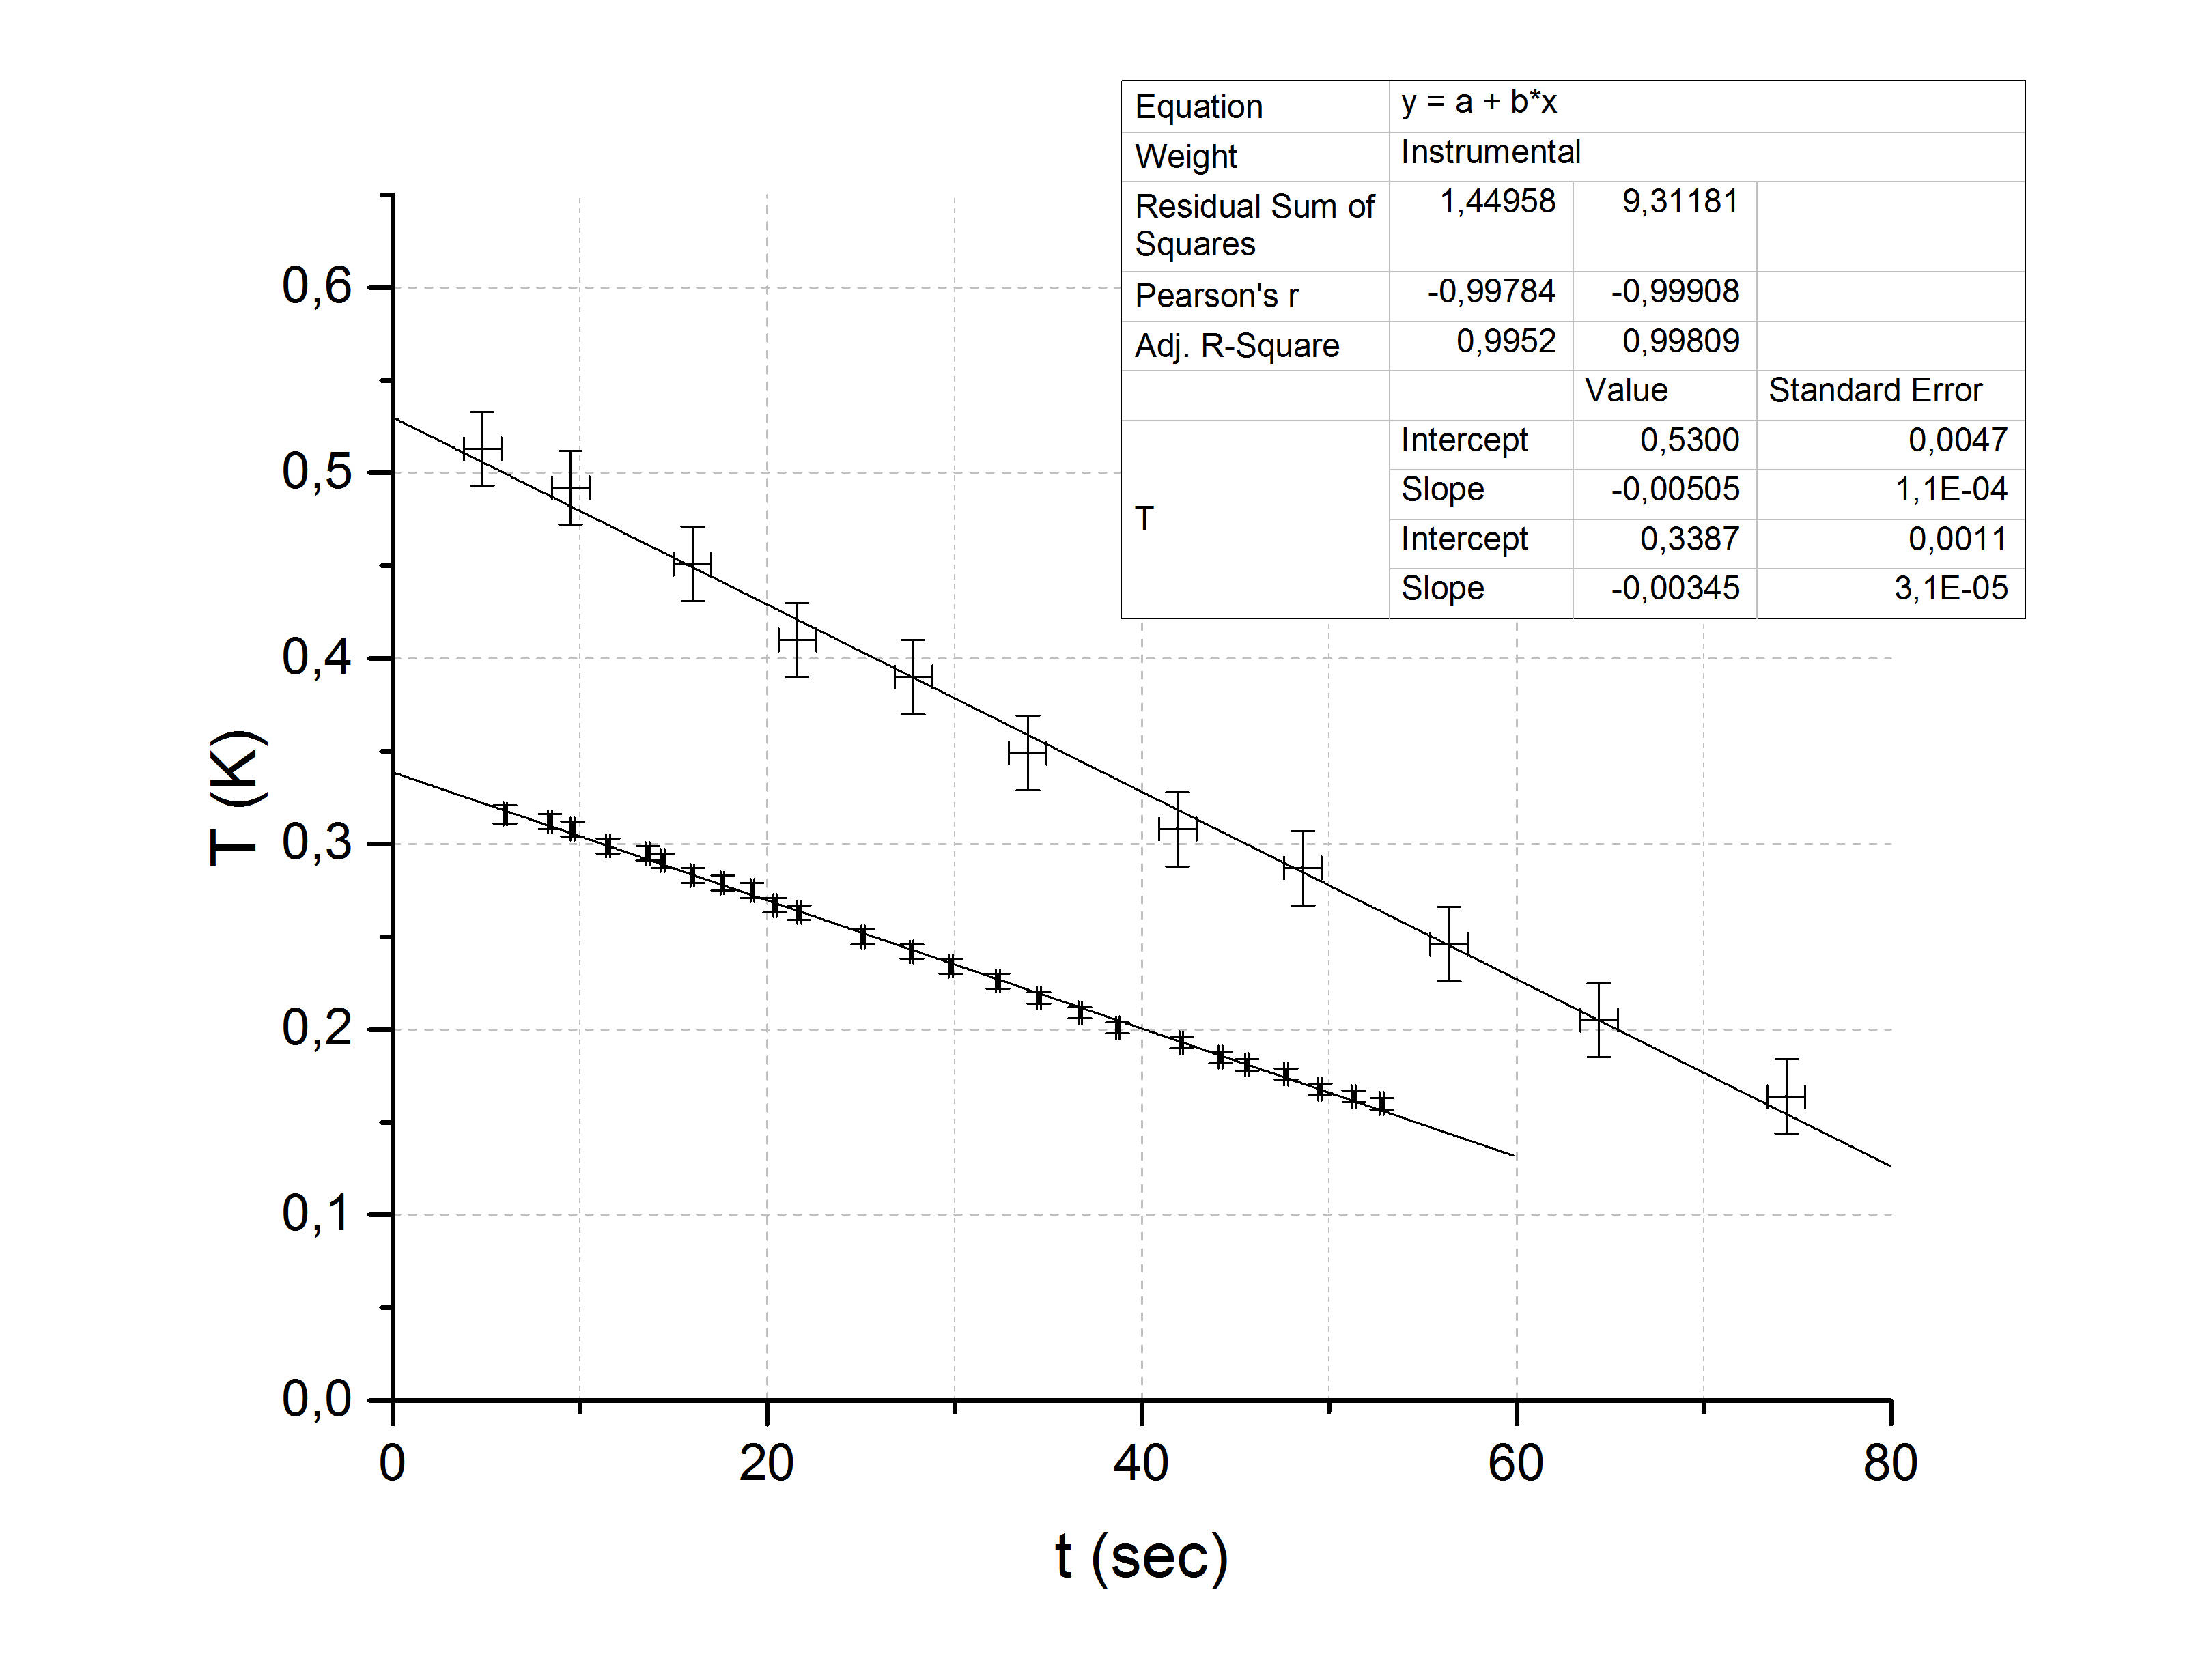
\includegraphics[width=150mm]{graph2_2.jpg}
\caption{Зависимость разницы температур резинки и воздуха от времени в 1-ом и 3-ем экспериментах при остывании резины после её резкого растяжения и экстраполяция этой зависимости до начального момента времени}
\end{figure}
 
\end{document} % конец документа